
\documentclass[tikz,border=10pt]{standalone} 
 
\usepackage{tikz} 
\usetikzlibrary{arrows.meta,positioning,calc,shapes.geometric} 
 
%--- custom colours ---------------------------------------------------- 
\definecolor{evtText}{HTML}{4F81BD}   % blue 
\definecolor{evtStatic}{HTML}{3CB4C8} % cyan 
\definecolor{evtTemp}{HTML}{F4A742}   % orange 
\definecolor{evtAdapt}{HTML}{D94A38}  % red 
 
\begin{document} 
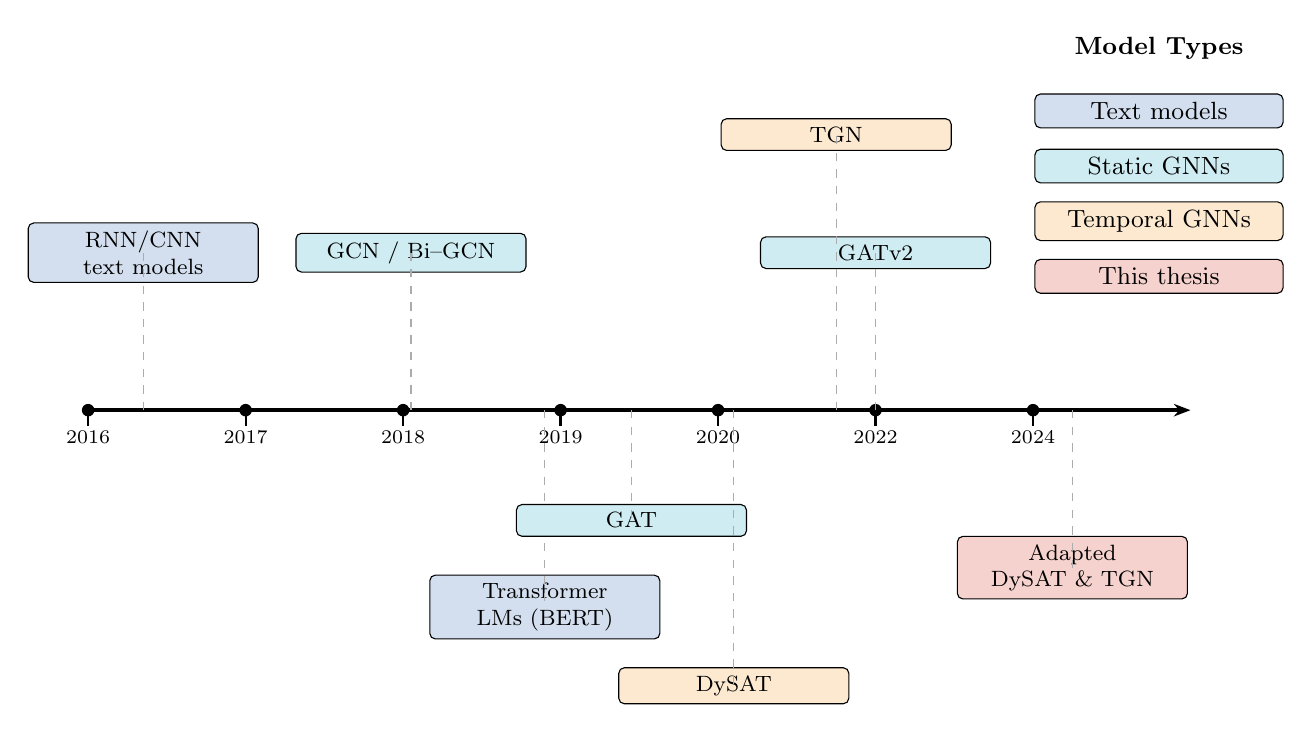
\begin{tikzpicture}[ 
    >=Stealth, 
    timeline/.style={ultra thick,-{Stealth[length=6pt]}}, 
    tick/.style={black, thick}, 
    dot/.style={circle,inner sep=1.6pt,fill=black}, 
    event/.style={draw, rounded corners=2pt, font=\footnotesize,  
                  inner xsep=6pt, inner ysep=3pt, 
                  text width=2.5cm, align=center}, % Increased width
    legend/.style={draw, rounded corners=2pt, font=\small,
                  inner xsep=5pt, inner ysep=3pt,
                  text width=2.8cm, align=center}, % Wider legend boxes
    every node/.style={font=\small}, 
] 
 
%----------------------------------------------------------------------- 
% axis (extended for better spacing)
\draw[timeline] (0,0) -- (14,0); 
 
% year ticks + markers 
\foreach \X/\Yr in {0/2016,2/2017,4/2018,6/2019,8/2020,10/2022,12/2024} 
{ 
  \draw[tick] (\X,0) -- ++(0,-.20); 
  \node[below=4pt,font=\scriptsize] at (\X,0) {\Yr}; 
  \node[dot] at (\X,0) {}; 
} 
 
%----------------------------------------------------------------------- 
% Define coordinates for better control
% Upper events (positive y)
\coordinate (e1) at (0.7, 2.0);  % RNN/CNN
\coordinate (e3) at (4.1, 2.0);  % GCN
\coordinate (e5) at (10.0, 2.0); % GATv2
\coordinate (e7) at (9.5, 3.5);  % TGN

% Lower events (negative y)
\coordinate (e2) at (5.8, -2.5); % Transformer
\coordinate (e4) at (6.9, -1.4); % GAT
\coordinate (e6) at (8.2, -3.5); % DySAT
\coordinate (e8) at (12.5, -2.0); % Adapted
 
% Place event boxes and connectors
\node[event,fill=evtText!25] at (e1) {RNN/CNN text models}; 
\draw[dashed,gray!65] (0.7,0) -- (e1);

\node[event,fill=evtText!25] at (e2) {Transformer LMs (BERT)}; 
\draw[dashed,gray!65] (5.8,0) -- (e2);

\node[event,fill=evtStatic!25] at (e3) {GCN / Bi--GCN}; 
\draw[dashed,gray!65] (4.1,0) -- (e3);

\node[event,fill=evtStatic!25] at (e4) {GAT}; 
\draw[dashed,gray!65] (6.9,0) -- (e4);

\node[event,fill=evtStatic!25] at (e5) {GATv2}; 
\draw[dashed,gray!65] (10.0,0) -- (e5);

\node[event,fill=evtTemp!25] at (e6) {DySAT}; 
\draw[dashed,gray!65] (8.2,0) -- (e6);

\node[event,fill=evtTemp!25] at (e7) {TGN}; 
\draw[dashed,gray!65] (9.5,0) -- (e7);

\node[event,fill=evtAdapt!25] at (e8) {Adapted DySAT \& TGN}; 
\draw[dashed,gray!65] (12.5,0) -- (e8);
 
%----------------------------------------------------------------------- 
% Simplified legend matching the image
\begin{scope}[shift={(12.2,3.8)}] 
  % Create legend title
  \node[font=\small\bfseries, align=center] at (1.4,0.8) {Model Types};
  
  % Legend items with single-line style
  \node[legend,fill=evtText!25] (L1) at (1.4,0) {Text models}; 
  \node[legend,fill=evtStatic!25] at (1.4,-0.7) {Static GNNs}; 
  \node[legend,fill=evtTemp!25] at (1.4,-1.4) {Temporal GNNs}; 
  \node[legend,fill=evtAdapt!25] at (1.4,-2.1) {This thesis}; 
\end{scope}
 
\end{tikzpicture} 
\end{document}